\documentclass[11pt]{article}
\usepackage[hmargin={1in},vmargin={1in,1in}]{geometry}   
\geometry{letterpaper}            
\usepackage[parfill]{parskip}
\usepackage{color,graphicx}
\usepackage{setspace}
\usepackage{amsmath}
\usepackage{amssymb}
\usepackage{textcomp}
\usepackage{linguex}
\usepackage{multirow}
\usepackage{pifont}
\usepackage{natbib}
\usepackage[normalem]{ulem}
\usepackage{wrapfig}

\usepackage{fancyhdr}
\lhead{Scontras, Degen \& Goodman}\chead{}\rhead{Adjective ordering}
\renewcommand{\headrulewidth}{.3pt}
\lfoot{}\cfoot{\thepage}\rfoot{}
\newcommand{\txtp}{\textipa}
\renewcommand{\rm}{\textrm}
\newcommand{\sem}[1]{\mbox{$[\![$#1$]\!]$}}
\newcommand{\lam}{$\lambda$}
\newcommand{\lan}{$\langle$}
\newcommand{\ran}{$\rangle$}
\newcommand{\type}[1]{\ensuremath{\left \langle #1 \right \rangle }}
\newcommand{\defeq}{$\mathrel{\mathop:}=$ }
\renewcommand{\and}{$\wedge$ }

\newcommand{\bex}{\begin{examples}}
\newcommand{\eex}{\end{examples}}
\newcommand{\bit}{\begin{itemize}}
\newcommand{\eit}{\end{itemize}}
\newcommand{\ben}{\begin{enumerate}}
\newcommand{\een}{\end{enumerate}}

\renewcommand{\bibsection}{}

\pagestyle{fancy}

\title{Adjective Ordering}
\author{Gregory Scontras, Judith Degen, and Noah D.~Goodman}
\date{\today}


\begin{document}

\thispagestyle{plain}

\maketitle

\begin{abstract}
	Here is the abstract
\end{abstract}

\tableofcontents

\section{Introduction}

Background on adjective ordering preferences

\subsection{English}

\subsection{Cross-linguistic stability}


\section{Corpus work} \label{corpus}

\begin{figure}[h!]
	\centering
	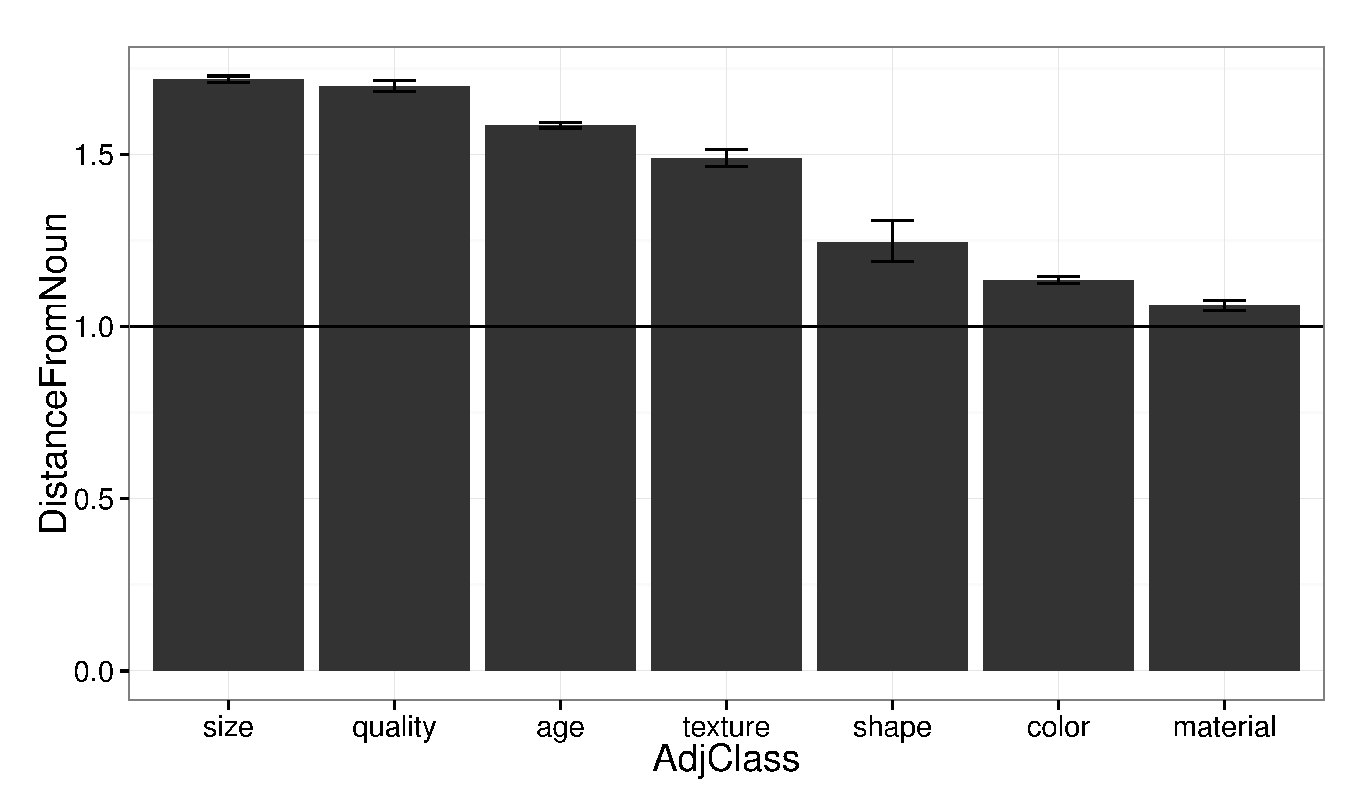
\includegraphics[width=.8\linewidth]{plots/distance_from_noun.eps}
	\caption{Average distance from noun by adjective class for cases with at least two modifying adjectives (39,199 cases).}\label{distance-from-noun}
\end{figure}

Based on the average distance-from-noun scores calculated in Fig.~\ref{distance-from-noun}, we may infer the ordering preferences in \ref{inferred-order-preferences}.

\ex. \label{inferred-order-preferences}
\emph{Adjective order preferences inferred from corpus counts (Fig.~\ref{distance-from-noun}}):\\
size $\geq$ quality $>$ age $>$ texture $>$ shape $>$ color $>$ material

\section{Experiments}


\subsection{Experiment 1: Subjectivity}

\subsubsection{Participants}

\subsubsection{Design and methods}


\begin{table}
	\centering
	\caption{Adjectives and nouns used in experimental stimuli.}\label{stim-table}
	\begin{tabular}{llccllc||cll}\hline
		\textsc{adjective} & \textsc{class} &&&\textsc{adjective} & \textsc{class} &&& \textsc{noun} & \textsc{class}\\\hline
		good	&	quality	&&&					old	&	age	&&&	apple	&	food	\\
		bad	&	quality	&&&					new	&	age	&&&	banana	&	food	\\
		round	&	shape	&&&					rotten	&	age	&&&	carrot	&	food	\\
		square	&	shape	&&&					fresh	&	age	&&&	cheese	&	food	\\
		big	&	size	&&&	red	&	color	&&&	tomato	&	food	\\
		small	&	size	&&&					yellow	&	color	&&&	chair	&	furniture	\\					
		huge	&	size	&&&					green	&	color	&&&	couch	&	furniture	\\
		tiny	&	size	&&&					blue	&	color	&&&	fan	&	furniture	\\					
		short	&	size	&&&					purple	&	color	&&&	TV	&	furniture	\\					
		long	&	size	&&&					brown	&	color	&&&	desk	&	furniture	\\					
		smooth	&	texture	&&&					wooden	&	material	&&&	\\								
		hard	&	texture	&&&					plastic	&	material	&&&		\\									
		soft	&	texture	&&&					metal	&	material	&&&		 
	\end{tabular}
\end{table}

\subsubsection{Predictions}

\subsubsection{Results}

\subsubsection{Discussion}


\subsection{Experiment 2: Ordering preferences}

We have so far established a connection between adjective subjectivity (measured by faultless disagreement scores in Expt.~1) and adjective proximity to nouns (obtained from corpus counts in Section \ref{corpus}). Our next task is to verify the adjective ordering preferences that we have inferred from the corpus and from the literature on the topic, and to evaluate the predictive power of subjectivity in determining adjective order. To that end, we elicited naturalness judgments on adjective-adjective-noun object descriptions, permuting the relative order of adjectives. We then compared these naturalness judgments with the faultless disagreement scores from the previous experiment.

\subsubsection{Participants}

We recruited 50 participants through Amazon.com's Mechanical Turk crowd-sourcing service. Participants were compensated for their participation.

\subsubsection{Design and methods}

Participants were asked to indicate which of two descriptions of an object sounded more natural. Each description featured a noun modified by two adjectives, for example ``the red small chair'' or ``the small red chair''. Description pairs contained the same words, with relative adjective order reversed. Descriptions were random combinations of two adjectives and a noun from the list in Table \ref{stim-table} (compiled via the procedure described in Section \ref{corpus}), with the constraint that no description contained adjectives from the same adjective class.
On each trial, participants indicated which description sounded more natural by adjusting a slider whose endpoints were labeled with the competing descriptions; an example trial appears in Fig.~\ref{order-trial}.

\begin{figure}[h!]
	\centering
	\fbox{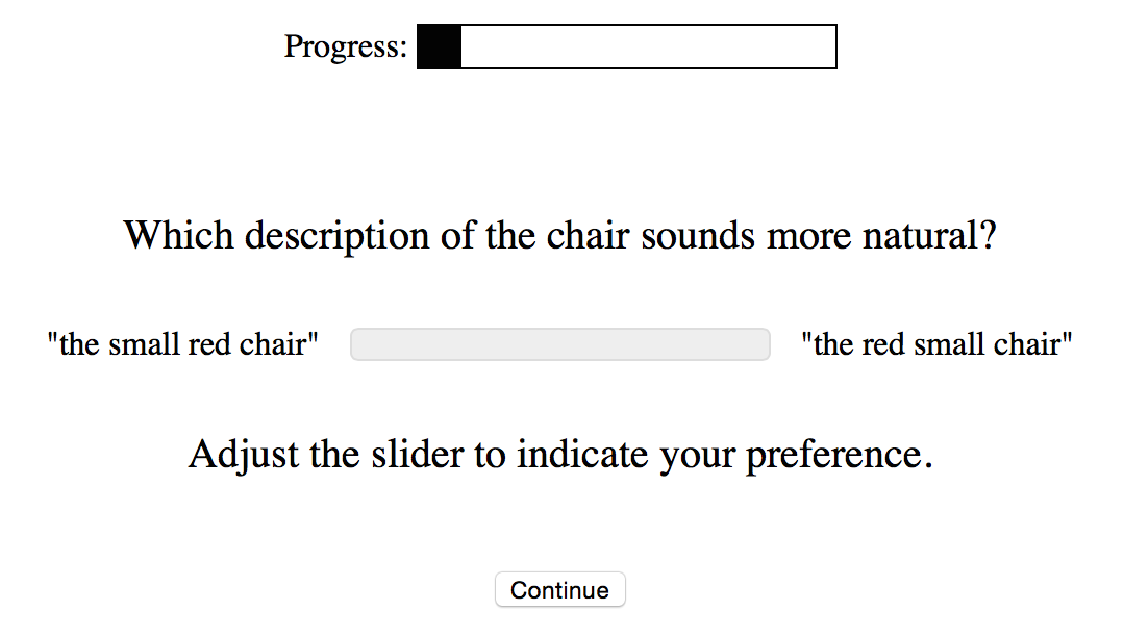
\includegraphics[width=.8\linewidth]{images/order_trial.eps}}
	\caption{Example trial from Expt.~1; participants indicated the more natural of two adjective-adjective-noun descriptions on a sliding scale.}\label{order-trial}
\end{figure}

Only native speakers of English with IP addresses located within the United States were included in the analyses; we analyzed data from 45 participants.

\subsubsection{Predictions}



\subsubsection{Results}

For each pair of adjective classes, we determine the preferred ordering on the basis of the ratio of ratings for the each order. Ratio scores greater than 1 indicate the preferred ordering; these ratio scores for the preferred orderings are plotted in Fig.~\ref{order-ratio}.

\begin{figure}[h!]
	\centering
	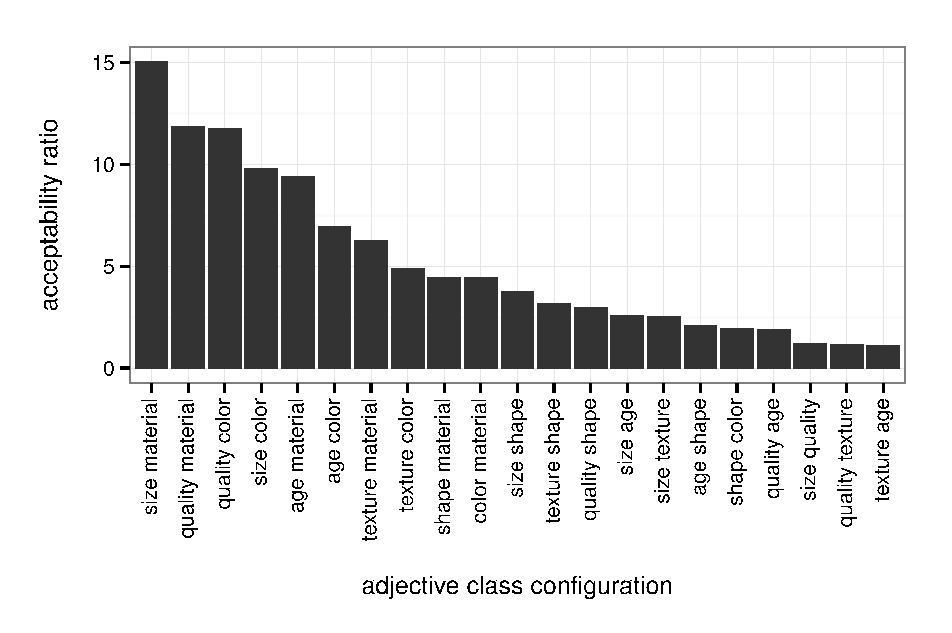
\includegraphics[width=.8\linewidth]{plots/order_ratio.eps}
\caption{Accpetability ratios for the preferred adjective class orderings.}\label{order-ratio}
\end{figure}

On the basis of these preferred orderings, we may calculate the average distance from noun for each class, plotted in Fig.~\ref{class-distance}. Comparing Fig.~\ref{class-distance} with the corpus-based distance scores reported in Fig.~\ref{distance-from-noun} confirms the reliability of the current paradigm: we replicate near exactly the qualitative order of adjective class distance from noun. 

\begin{figure}[h!]
	\centering
	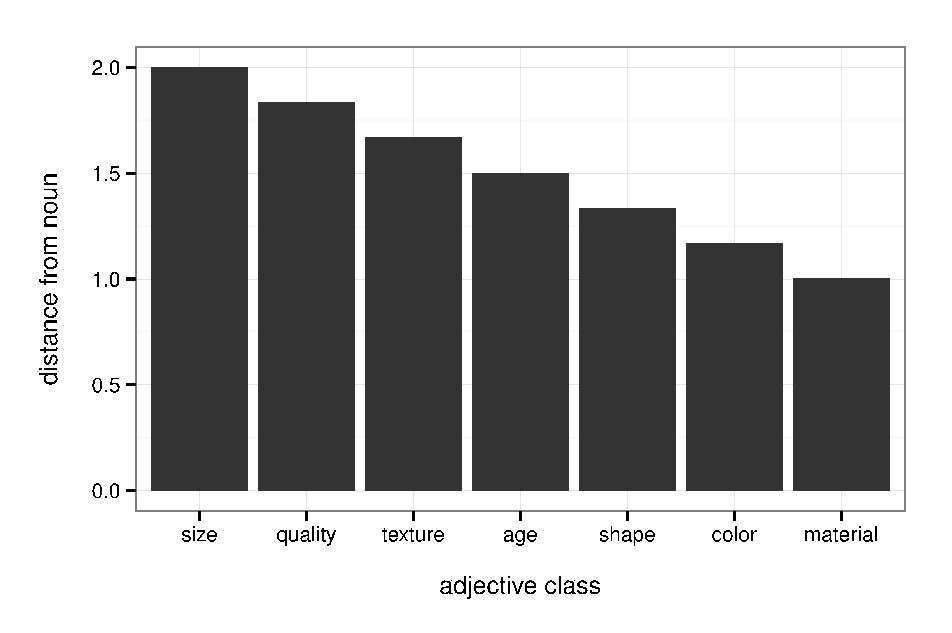
\includegraphics[width=.8\linewidth]{plots/class_distance.eps}
	\caption{Average distance from noun for each adjective class calculated from order preference ratings.}\label{class-distance}
\end{figure}

We may infer the order preferences in \ref{expt-inferred-order-preferences} (cf.~the preferences inferred from corpus counts in \ref{inferred-order-preferences} above).

\ex. \label{expt-inferred-order-preferences}
\emph{Adjective order preferences inferred from acceptability ratings (Fig.~\ref{class-distance})}:\\
size $>$ quality $>$ age $>$ texture $>$ shape $>$ color $>$ material

In addition to calculating preference ratios by class configurations, we also calculated preferred orderings for all of the specific adjective pairings. On the basis of how often an adjective from a given class occurred first in an adjective-adjective-noun configuration, we may infer the relative distance from the noun a given class prefers. Fig.~\ref{class-distance-by-adj} plots these average distance scores, where a value of 2 signals that a class's adjectives always occur first in preferred adjective-adjective-noun orderings, and a value of 1 indicates that a class's adjectives always occur second.

\begin{figure}[h!]
	\centering
	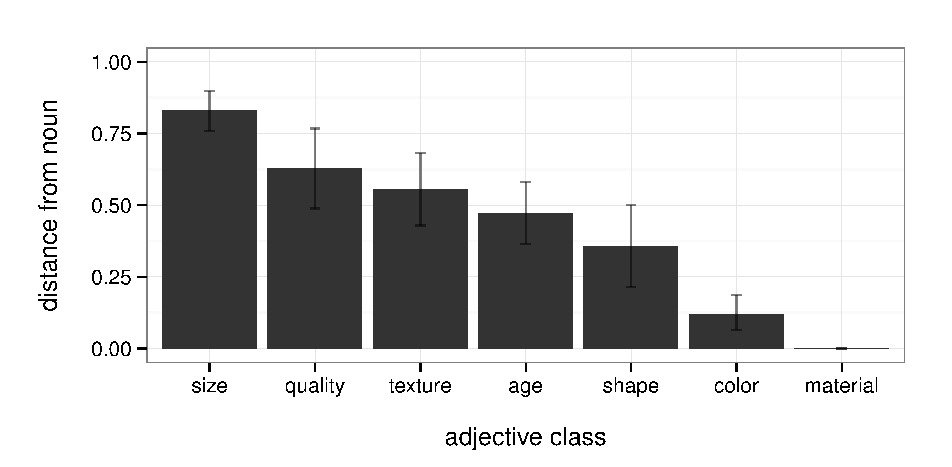
\includegraphics[width=.8\linewidth]{plots/class_distance_by_adj.eps}
	\caption{Average distance from noun for each adjective class by computing how often adjectives from that class occur first in preferred adjective-adjective-noun orderings.}\label{class-distance-by-adj}
\end{figure}

Finally, and most directly related to our hypothesis concerning adjective subjectivity in ordering preferences, we compared acceptability ratings from the current experiment with faultless disagreement scores from Expt.~1. To do so, we first calculated a difference score for each class configuration, \textsc{class1}--\textsc{class2}, subtracting the average faultless disagreement score for \textsc{class1} from the average faultless disagreement score for \textsc{class2}. Fig.~\ref{faultless-order} plots class configuration acceptability ratings against faultless disagreement difference scores.

\begin{figure}[h!]
	\centering
	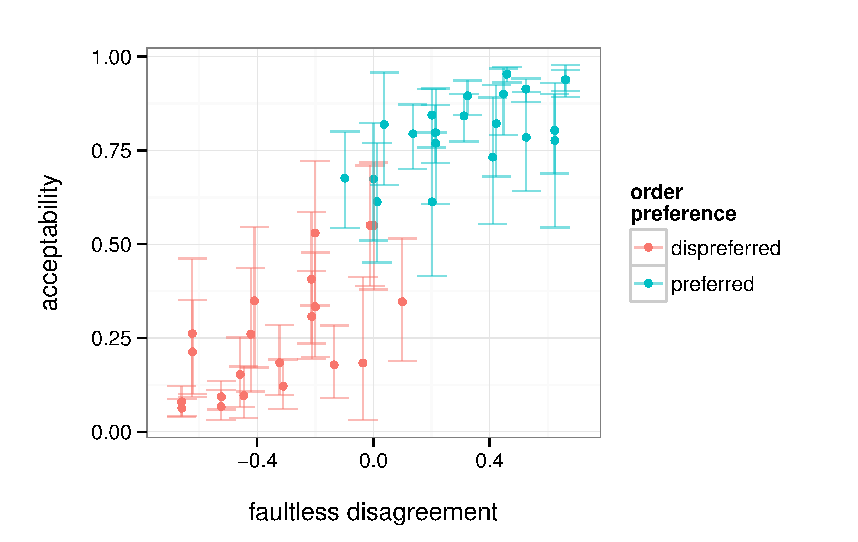
\includegraphics[width=.8\linewidth]{plots/faultless_order_preference.eps}
	\caption{By-class adjective order preferences plotted against difference in faultless disagreement.}\label{faultless-order}
\end{figure}

\subsubsection{Discussion}




\section{Possible accounts}


\subsection{Memory}

Forgetting account

\subsection{Syntax}

John Beavers spray/load work

\subsection{UID}

Different notions of informativity

\subsection{Flexibility}

\emph{Blue} is less subjective so I rarely speak of ``blue for X'', whereas more subjective and flexible \emph{good} is often spoken of in terms of ``good for Y''.


\section{General discussion}


\end{document}